our vector-based disaggregation approach utilizes more features including power levels, 
duration of on/off event, and partial or whole shape of on/off event.

Previous work may assume that we know the power levels of each electric device , 
or water flow rate of each water end use. 
Now, we assume that besides the aggregated data, we know the on/off events for each device for a period of time. 

The disaggregation framework for electricity and water disaggregation is illustrated in Figure \ref{fig_vectormotifmining}. 
For all the aggregated electricity or water data, 
we have the on/off events for a short period of time. 
Therefore we utilize these known events to search the aggregated data 
to extract the features, such as power levels or water flow rate level, 
the startup/shutdown duration, or startup or shutdown shape of each electricity device or water use end. 
In the next step, we apply window-variable motif mining to 
match those devices which have explicit usage level or startup duration. 
For devices with continuously variable load or variable water flow rate, 
we exploit dynamic time warping subsequence search. 
If a complete cycle of a device is matched by dynamic time warping subsequence search, 
then we can find this device. 
Otherwise, only partial of the startup/shutdown shape is used as a feature, 
dynamic time warping-based motif mining is applied again. 
In the last step, we recover each electric device or water use end from these motifs. 
%\begin{figure*}[!t]
%        \centering{
%		\includegraphics[width=6.4in]{figs/vectorMotifMining.pdf}
%                }
%        \caption{
%	Vector-based motif mining
%}
%        \label{fig_vectormotifmining}
%\end{figure*}

\begin{figure}[!t]
\centering
\includegraphics[width=0.5\textwidth]{multidisaggfigs/vectorMotifMining.pdf}
\caption{Vector-based motif mining}
\label{fig_vectormotifmining}
\end{figure}
